\documentclass{lab}

\title{Lab \# 1. Location Tech} % Title

\author{Adan Abunaaj | adan@mit.edu \\ Artem Laptiev | laptiev@mit.edu \\\\ 6.1820} % Team # + Names, Class (RSS)

\date{\today} % Date for the report

\begin{document}

\maketitle

\newpage

\section{Accuracy Levels}

Unfortunately, iOS Location Manager doesn't provide a way to specify exact sensor to use for location updates. Instead, the user can only specify the desired accuracy level as means to limit unnecessary battery drain. For each accuracy level, the exact usage of sensors is unclear. However, GPS usually corresponds to the best accuracy level, while cell tower triangulation is used for the worst accuracy level.

We also try to prevent sensor fusion by turning an/off WiFi and Cellular Data (though we don't have enough data to prove the latter is effective) for corresponding experiments.

Here's a table with the sensors used and corresponding chosen accuracy level:

\begin{table}[h!]
    \centering
    \begin{tabular}{|c|c|}
        \hline
        \textbf{Sensor} & \textbf{Accuracy Level} \\ \hline
        GPS & kCCLLocationAccuracyBestForNavigation \\ \hline
        Wifi & kCCLLocationAccuracyHundredMeters \\ \hline
        Cell & kCLLocationAccuracyThreeKilometers \\ \hline
    \end{tabular}
    \caption{Sensors and Accuracy Levels}
    \label{tab:accuracy}
\end{table}

\section{Average Estimated Distances}

We ran a total of 6 trials. Here's a table with the average estimated distances for each trial, error, and number of samples:

\begin{table}[h!]
    \centering
    \begin{tabular}{|c|c|c|c|}
        \hline
        \textbf{Sensor} & \textbf{Average Distance, m} & \textbf{Error, m} & \textbf{NSamples} \\ \hline
        Cellular (wifi is off) & 266.54 & 225.96 & 9 \\ \hline
        Cellular (wifi is off) & 645.07 & 152.57 & 15 \\ \hline
        Cellular (wifi is on) & 671.73 & 179.23 & 110 \\ \hline
        Wifi (cell is off) & 964.39 & 471.89 & 64 \\ \hline
        Wifi (cell is off) & 553.21 & 60.71 & 59 \\ \hline
        GPS & 559.54 & 67.04 & 276 \\ \hline
    \end{tabular}
    \caption{Estimated Distances for each of 6 trials}
    \label{tab:distances}
\end{table}

Judging by the number of samples in Cellular trial w/ WiFi on, we can conclude that the sensor fusion is indeed happening. So we discard this trial when computing averages.

One of the WiFi trials has a very high error. We keep it only for the lack of abundant data.


\begin{figure}[h]
\begin{center}
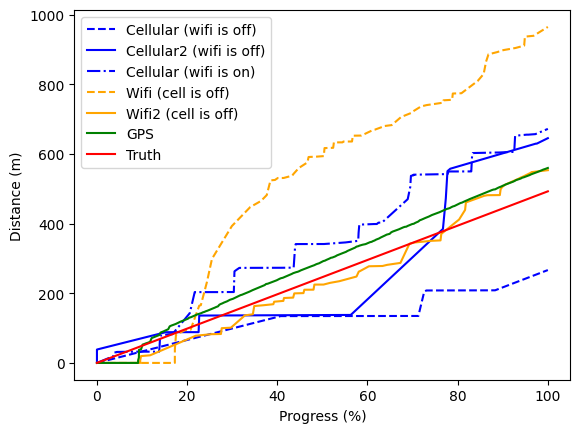
\includegraphics[width=0.65\textwidth]{images/distances.png} 
\caption{Estimated Distances for each of 6 trials}
\end{center}  
\end{figure}

\begin{table}[h!]
  \centering
  \begin{tabular}{|c|c|c|c|}
      \hline
      \textbf{Sensor} & \textbf{Average Distance} & \textbf{Error} & \textbf{NSamples} \\ \hline
      Cellular & 455.80 & 189.26 & 12.0 \\ \hline
      Wifi & 758.80 & 266.30 & 61.5 \\ \hline
      GPS & 559.54 & 67.04 & 276 \\ \hline
  \end{tabular}
  \caption{Average Distances}
  \label{tab:averages}
\end{table}


\section{Maps of the Points/Trajectories}

The figures 2, 3, and 4 are the maps of the most accurate trials for Cellular, Wifi, and GPS respectively.

\begin{figure}[h]
\begin{center}
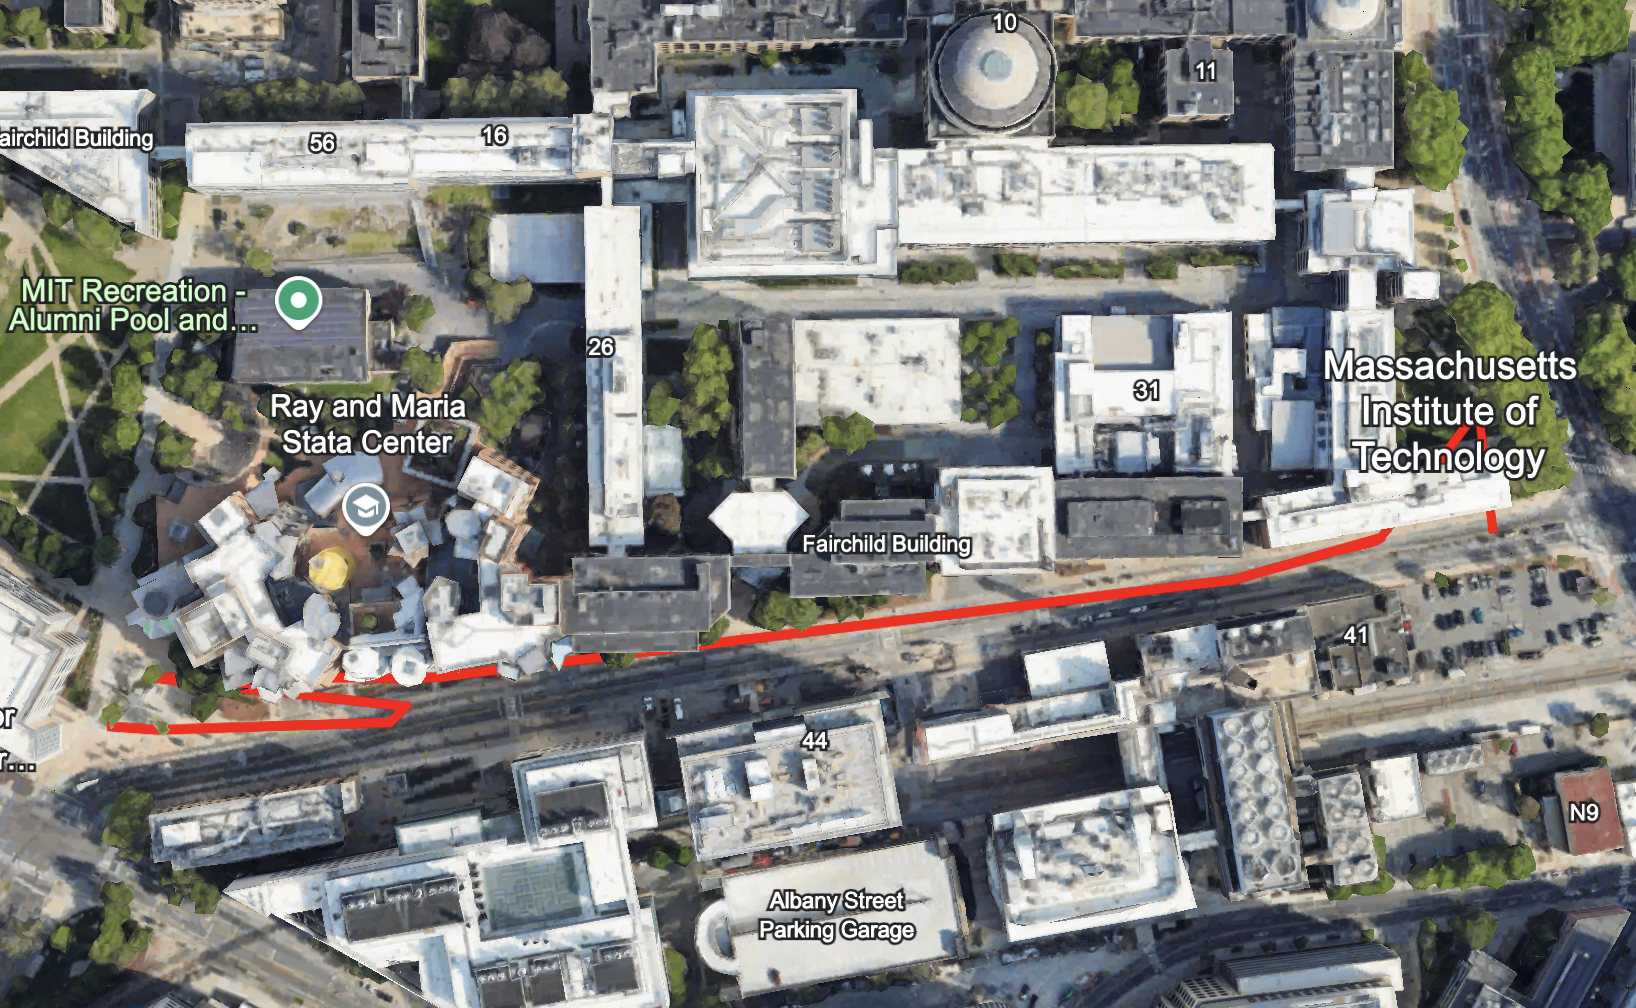
\includegraphics[width=0.65\textwidth]{images/cellular2.png}
\caption{Cellular}
\end{center}
\end{figure}

\begin{figure}[h]
\begin{center}
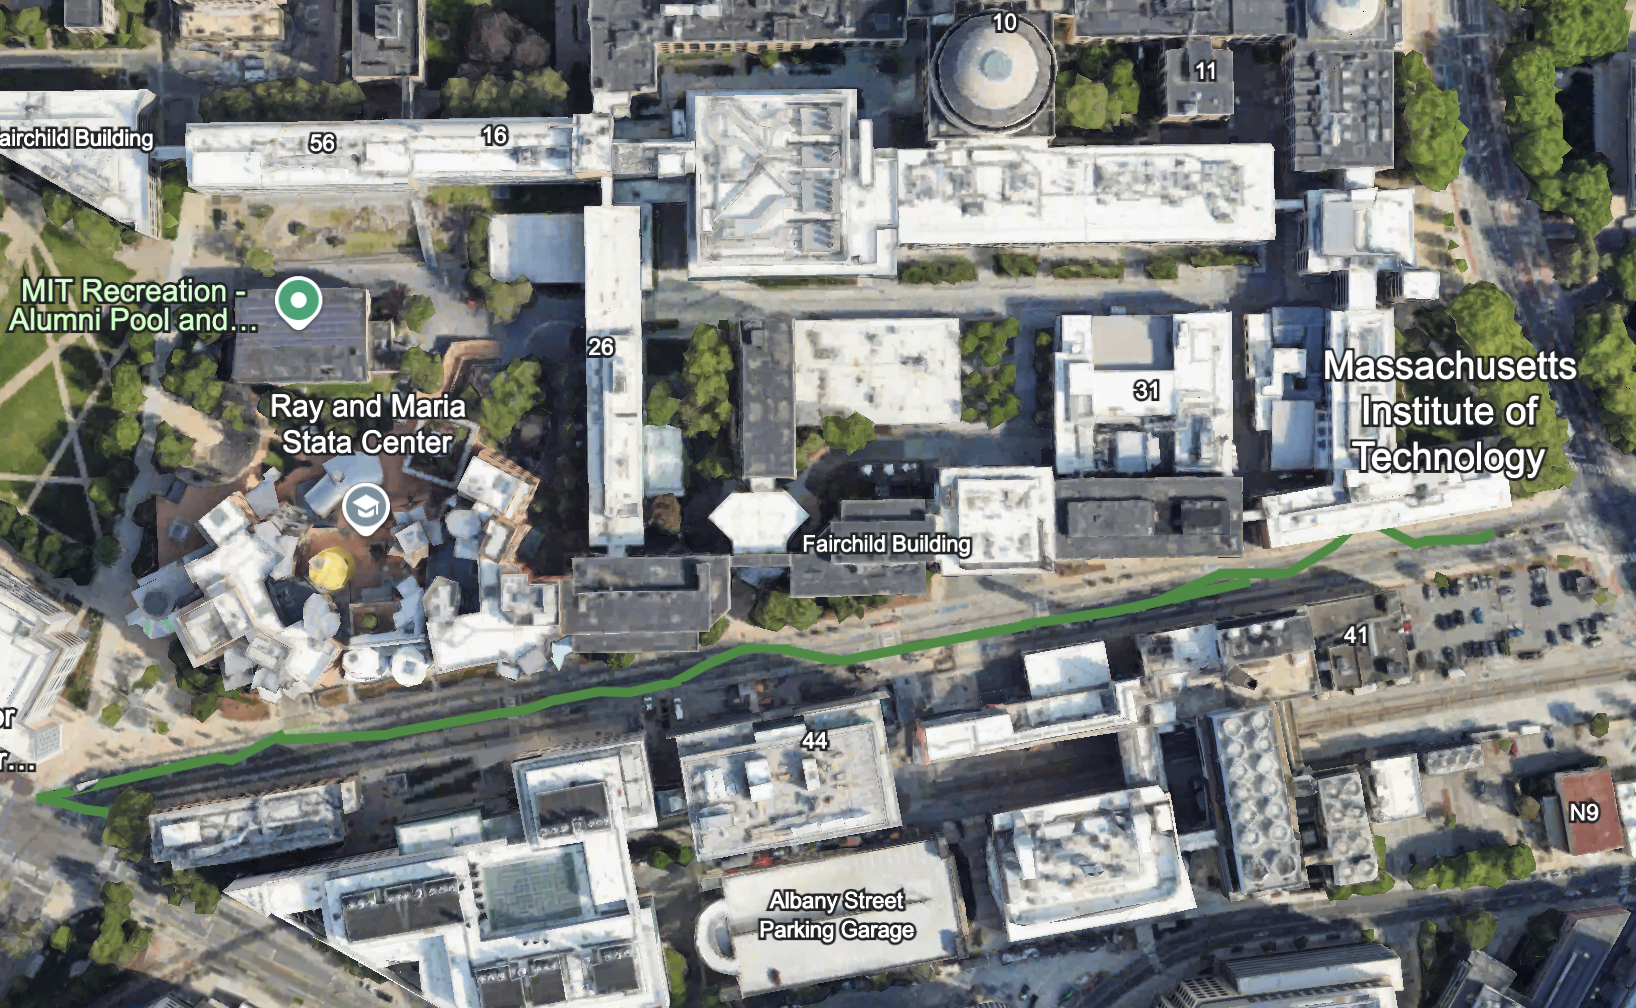
\includegraphics[width=0.65\textwidth]{images/wifi2.png}
\caption{Wifi}
\end{center}
\end{figure}

\begin{figure}[h]
\begin{center}
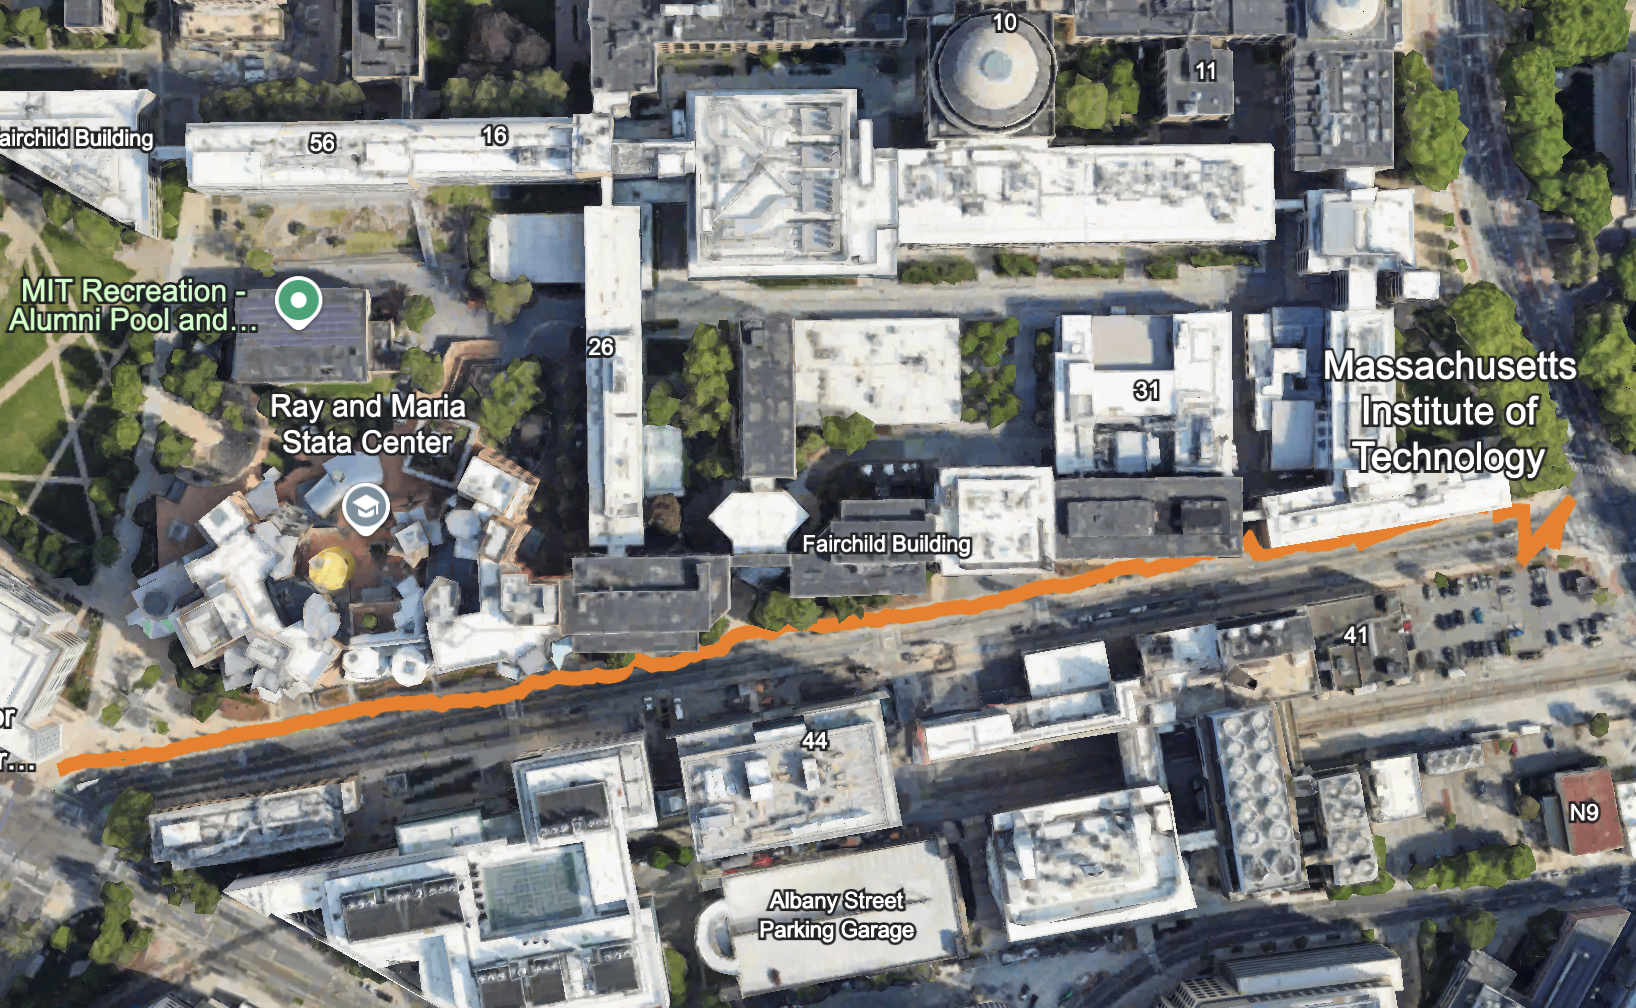
\includegraphics[width=0.65\textwidth]{images/gps.png}
\caption{GPS}
\end{center}
\end{figure}

\section{Plots of the Battery Drain}

\section{Time spent}

Time spent:

% list of items:
\begin{itemize}
  \item Task 1: $\leq 1$ hour
  \item Task 2, data collection: = 1 hour
  \item Task 2, data analysis + writeup: = 3 hours
\end{itemize}


\end{document}

